\documentclass[11pt]{article}

\usepackage[margin=1in]{geometry}
\usepackage{amsmath,amssymb,amsthm}
\usepackage{graphicx}
\usepackage{booktabs}
\usepackage{caption}
\usepackage{array}
\usepackage{xcolor}
\usepackage[hidelinks]{hyperref}
\usepackage{enumitem}
\usepackage{tabularx}
\usepackage{microtype}

% Numbering: every displayed equation numbered
\numberwithin{equation}{section}
\setlength{\parskip}{4pt}

% Supplementary figures: S1, S2, S3, ...  (Daniel: figures consistent S1 upward)
\renewcommand{\thefigure}{S\arabic{figure}}

\title{\bfseries Supplementary Materials\\
\large Seizure Forecasting and Crash Risk Analysis}
\author{}
\date{\today}

\begin{document}
\maketitle
\tableofcontents
\bigskip

\section{Overview}
\label{sec:overview}

This appendix gives the full model, the parameter derivations, the main result, the
sensitivity analyses, and the reproducibility instructions for the main paper.
All calculations are analytic (closed-form); the accompanying Jupyter notebook
\texttt{crashes\_vs\_TiW.ipynb} reproduces every figure and every number in this document.

We quantify the trade-off between seizure-forecasting accuracy (AUC), driving exposure,
and the driving restrictions required to maintain fatal crash risk at or below a safety
threshold of approximately $6\times$ baseline, corresponding to BAC $\approx 0.05$--$0.07\%$
for adult drivers. This benchmark aligns with the $0.05\%$ BAC standard used in Utah
and most European countries, more conservative than the $0.08\%$ BAC limit in
$49$ U.S.\ states.

\paragraph{Key modeling feature.}
Relative fatal crash risk on forecasted ``safe'' days is computed using a per-hour
fatal-crash baseline $\lambda_f \approx 4.5 \times 10^{-7}\,\text{hr}^{-1}$ and a
conditional probability $q_f = P(\text{fatal crash} \mid \text{seizure while driving}) =
0.02$ (central estimate; range $0.005$--$0.05$ in sensitivity analyses).
The probability that a seizure coincides with driving scales as $D/24$ for daily driving
duration $D$; however, because both seizure-related and baseline risk scale with
exposure, the relative-risk benchmark remains approximately invariant to $D$
(Section~\ref{sec:crash-risk}).

\paragraph{Key findings.}
Patients with infrequent seizures ($\le 1$/year) approach unrestricted driving even at
low AUC, whereas patients with frequent seizures require AUC $\ge 0.90$ to drive
meaningfully. At AUC $0.90$ and $1$\,hr/day driving, weekly seizures permit $\approx 53$
days/year, monthly seizures $\approx 182$, and yearly seizures $\approx 365$.
These results depend little on driving duration but moderately on $q_f$
(Section~\ref{sec:sensitivity}).

\section{Model and Methods}
\label{sec:methods}

This section builds the model in the order it is computed: forecasting model, seizure
prior, Bayesian posterior on forecast-safe days, fatal-crash-risk model, safety
threshold, and conversion to driving days.

\subsection{Binormal ROC Framework}
\label{sec:binormal}

We model the forecasting algorithm's output as a scalar score $S$ generated by one of two
normal distributions, depending on whether the day is a seizure day.

\paragraph{Variable definitions used throughout this appendix.}
\begin{itemize}[leftmargin=2em,itemsep=2pt]
  \item $S$: the forecasting algorithm's output score on a given day.
  \item $m$: the separation between the seizure and non-seizure score distributions
        (larger $m$ means the algorithm discriminates better).
  \item $t$: the operating threshold; the algorithm warns \emph{unsafe to drive} when
        $S > t$ and forecasts \emph{safe to drive} when $S \le t$.
  \item $\Phi(\cdot)$: the cumulative distribution function (CDF) of the standard
        normal distribution $N(0,1)$.
  \item $\Phi^{-1}(\cdot)$: the inverse standard-normal CDF (quantile function).
  \item $\mathrm{AUC}$: area under the receiver operating characteristic curve.
\end{itemize}

The forecast score is distributed as
\begin{equation}
S \sim N(0, 1) \quad \text{on a non-seizure day}, \qquad
S \sim N(m, 1) \quad \text{on a seizure day}.
\label{eq:score-dist}
\end{equation}
Under this equal-variance binormal model, the separation $m$ relates to AUC by
\begin{equation}
m = \sqrt{2}\;\Phi^{-1}(\mathrm{AUC}).
\label{eq:m-auc}
\end{equation}

For threshold $t$ applied to the score, the sensitivity (true-positive rate) and false-positive
rate are
\begin{equation}
\mathrm{Sensitivity} = P(S > t \mid \text{seizure}) = 1 - \Phi(t - m) = \Phi(m - t),
\label{eq:sensitivity}
\end{equation}
\begin{equation}
\mathrm{FPR} = P(S > t \mid \text{no seizure}) = 1 - \Phi(t).
\label{eq:fpr}
\end{equation}

Figure~\ref{fig:S1} illustrates the model geometrically: the two score distributions,
the threshold $t$, the separation $m$, and the regions whose probability mass equals
sensitivity (\ref{eq:sensitivity}) and FPR (\ref{eq:fpr}). Section~\ref{sec:roc-shape}
tests robustness to alternative ROC shapes.

\begin{figure}[h!]
  \centering
  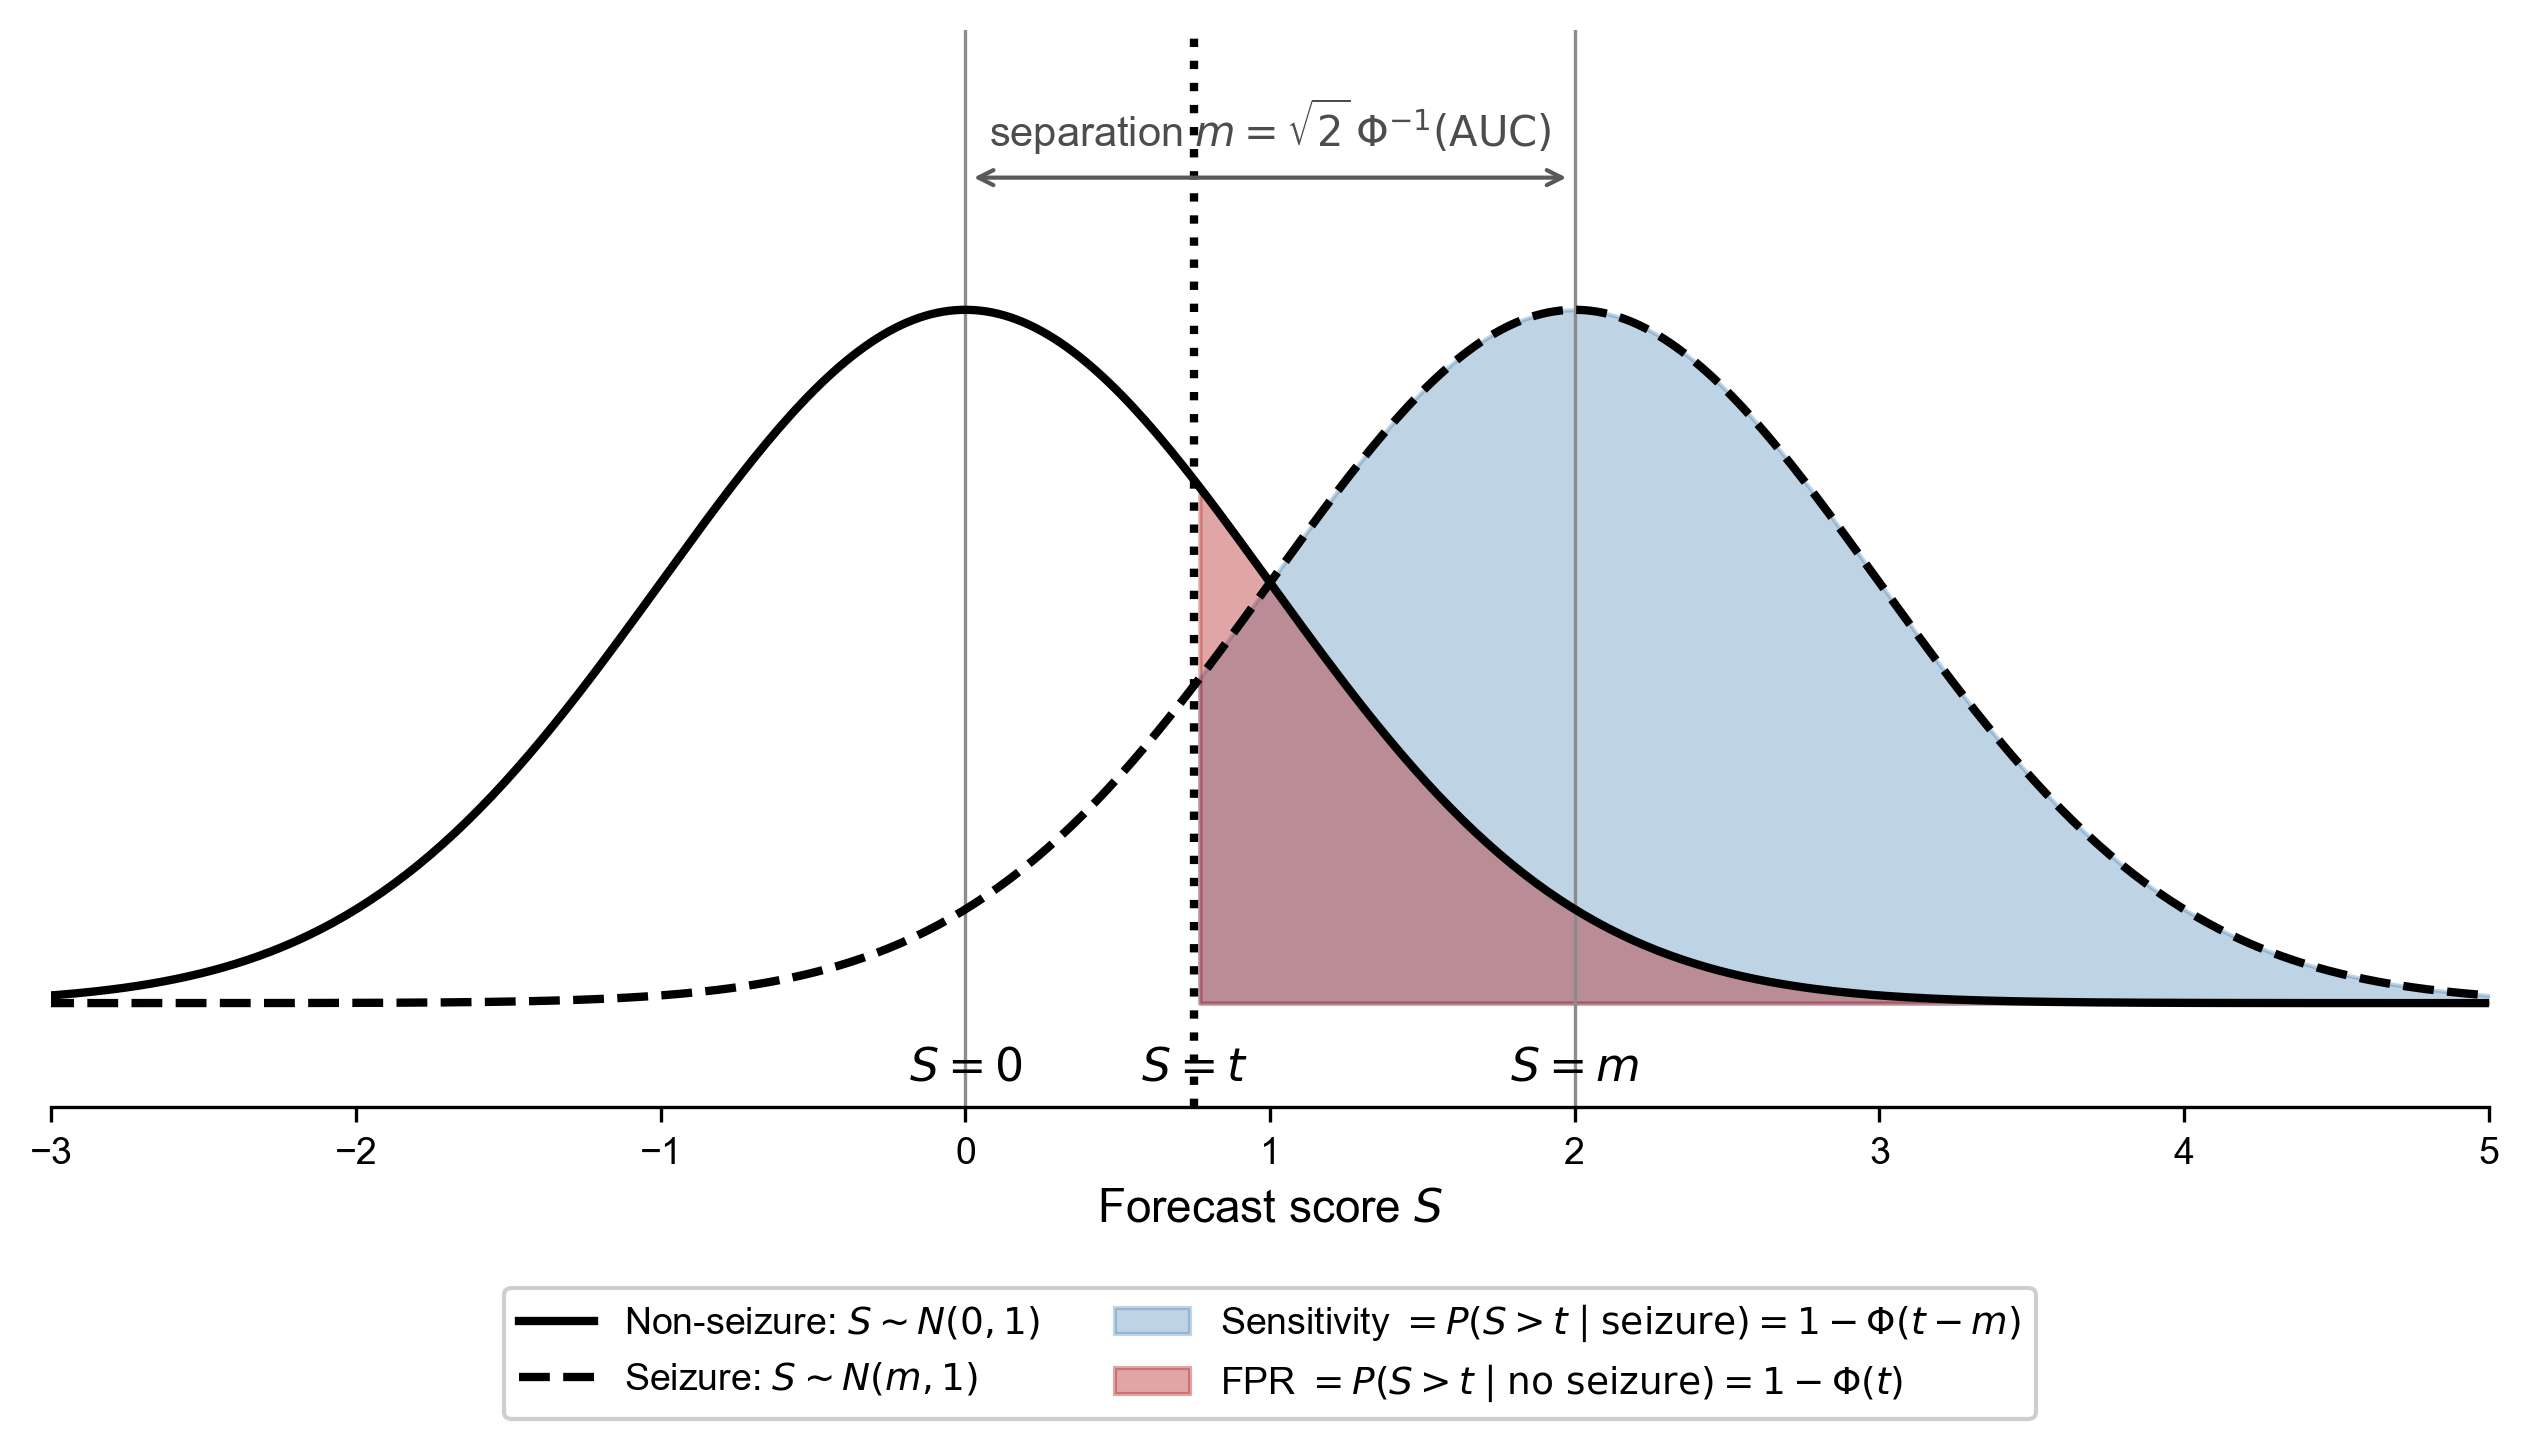
\includegraphics[width=0.9\textwidth]{Figure_S1.png}
  \caption{\textbf{Binormal forecast model.} Score distributions on non-seizure days
  ($S\sim N(0,1)$, solid) and seizure days ($S\sim N(m,1)$, dashed). The threshold $t$
  (dotted vertical) defines the decision boundary; sensitivity (blue) and FPR (red) are
  the probability masses right of $t$ under the seizure and non-seizure distributions.
  Separation parameter $m$ relates to AUC via Equation~\ref{eq:m-auc}.}
  \label{fig:S1}
\end{figure}

\subsection{Daily Seizure Probability}
\label{sec:daily-prob}

For a patient with average seizure rate $R$ (seizures per day), the daily seizure
probability under a Poisson process is
\begin{equation}
p = 1 - e^{-R}.
\label{eq:daily-prob}
\end{equation}
\begin{center}
\begin{tabular}{lcc}
\toprule
Frequency & $R$ & $p$ \\
\midrule
1 seizure / week  & $1/7$   & $\approx 0.133$ \\
1 seizure / month & $1/30$  & $\approx 0.033$ \\
1 seizure / year  & $1/365$ & $\approx 0.0027$ \\
\bottomrule
\end{tabular}
\end{center}

The Poisson mapping is used only to translate an average rate into a daily probability;
the analysis is otherwise agnostic to the temporal structure of seizure risk.

\subsection{Posterior Seizure Probability on Forecast-Safe Days}
\label{sec:posterior}

When a patient drives on a forecast-safe day (one for which the algorithm output
$S \le t$), the residual crash risk is driven by the posterior probability of a seizure
given that negative forecast. By Bayes' theorem,
\begin{equation}
P(\text{seizure} \mid \text{forecast safe}) \;=\;
\frac{P(\text{forecast safe} \mid \text{seizure}) \cdot p}
     {P(\text{forecast safe} \mid \text{seizure}) \cdot p
      + P(\text{forecast safe} \mid \text{no seizure}) \cdot (1 - p)}.
\label{eq:bayes-1}
\end{equation}

We obtain the two conditional probabilities in (\ref{eq:bayes-1}) directly from
sensitivity and FPR by complementation:
\begin{align}
P(\text{forecast safe} \mid \text{seizure})
   &\;=\; 1 - P(\text{forecast unsafe} \mid \text{seizure}) \;=\; 1 - \mathrm{Sensitivity}, \label{eq:safe-seiz}\\
P(\text{forecast safe} \mid \text{no seizure})
   &\;=\; 1 - P(\text{forecast unsafe} \mid \text{no seizure}) \;=\; 1 - \mathrm{FPR}. \label{eq:safe-noseiz}
\end{align}

Substituting (\ref{eq:safe-seiz})--(\ref{eq:safe-noseiz}) into (\ref{eq:bayes-1}) and
using the binormal expressions for sensitivity (\ref{eq:sensitivity}) and FPR
(\ref{eq:fpr}) gives
\begin{equation}
P(\text{seizure} \mid \text{forecast safe})
\;=\;
\frac{(1 - \mathrm{Sensitivity})\, p}
     {(1 - \mathrm{Sensitivity})\, p + (1 - \mathrm{FPR})\,(1 - p)}
\;=\;
\frac{\Phi(t - m)\, p}{\Phi(t - m)\, p + \Phi(t)\,(1 - p)}.
\label{eq:posterior}
\end{equation}

\subsection{Fatal Crash Risk and the Relative-Risk Derivation}
\label{sec:crash-risk}

\paragraph{Parameters used in this subsection.}
We use the parameters in Table~\ref{tab:params} throughout the crash-risk derivation.

\begin{table}[h!]
\caption{Crash-risk model parameters.}
\label{tab:params}
\centering
\renewcommand{\arraystretch}{1.25}
\begin{tabularx}{\linewidth}{lXcX}
\toprule
Symbol & Meaning & Value & Source \\
\midrule
$\lambda_f$ & Baseline fatal-crash rate per hour of sober driving
            & $4.5\times 10^{-7}\,\text{hr}^{-1}$
            & NHTSA \emph{Passenger Vehicles 2023} + FHWA \emph{Highway Statistics 2023}
              + AAA \emph{American Driving Survey 2023}
              (derivation in this section) \\
$q_f$       & $P(\text{fatal crash} \mid \text{seizure while driving})$
            & $0.02$ central; range $0.005$--$0.05$
            & Inferred severity parameter; see Section~\ref{sec:qf-sensitivity} \\
$D$         & Driving hours per day & $0.5,\ 1,\ 2$ & --- \\
$\pi$       & $P(\text{seizure} \mid \text{forecast safe})$
            & From Eq.~(\ref{eq:posterior}) & --- \\
\bottomrule
\end{tabularx}
\end{table}

\paragraph{Baseline per-day fatal-crash risk.}
Given $D$ hours of driving per day and a per-hour baseline rate $\lambda_f$, a sober
driver faces a per-day baseline fatal-crash risk of
\begin{equation}
B(D) \;=\; D \cdot \lambda_f.
\label{eq:baseline-day}
\end{equation}

\paragraph{Derivation of $\lambda_f$.}
NHTSA \emph{Passenger Vehicles 2023} reports $\sim 44{,}000$ passenger vehicles involved
in fatal crashes; FHWA \emph{Highway Statistics 2023} Table VM-1 reports $\sim 2.88$
trillion light-duty vehicle-miles travelled (VMT). The ratio is approximately
$1.5$ passenger-vehicle fatal-crash involvements per $10^{8}$ miles, i.e.\ $1.5\times 10^{-8}$
per mile. Converting per-mile to per-hour requires a driving speed: the AAA
\emph{American Driving Survey 2023} reports $\approx 29.1$ miles over $\approx 60.7$
minutes per driver per day, i.e.\ $\approx 29$ mph. Then
\begin{equation}
\lambda_f \;\approx\; 1.5\times 10^{-8}\,\text{mile}^{-1} \times 29\,\text{mph}
\;\approx\; 4.4 \times 10^{-7}\,\text{hr}^{-1}
\;\approx\; 4.5 \times 10^{-7}\,\text{hr}^{-1}.
\label{eq:lambda-derivation}
\end{equation}
(FHWA Table VM-1 supplies the VMT denominator only; the AAA survey provides driving
speed for the per-mile-to-per-hour conversion.) Because this baseline
incorporates all non-seizure causes of fatal crashes (distraction, weather, other
drivers), the model conservatively attributes this background risk to every driving day
regardless of seizure status.

\paragraph{Seizure-day fatal-crash risk.}
On a day when a seizure occurs, the per-day fatal-crash risk depends on whether the
seizure falls within the driving window. Assuming uniform seizure timing across the
$24$-hour day,
\begin{equation}
P(\text{fatal crash} \mid \text{seizure day})
\;=\; \frac{D}{24}\cdot q_f \;+\; \left(1 - \frac{D}{24}\right)\cdot B(D).
\label{eq:fatal-seiz-day}
\end{equation}
The first term captures seizures during driving; the second captures baseline risk when
the seizure occurs outside driving hours.

\paragraph{Forecast-safe-day fatal-crash risk.}
Let $\pi = P(\text{seizure} \mid \text{forecast safe})$ from Equation~\ref{eq:posterior}.
On a forecast-safe day, residual fatal-crash risk is
\begin{equation}
P(\text{fatal crash} \mid \text{forecast safe})
\;=\; \pi \cdot P(\text{fatal crash} \mid \text{seizure day})
\;+\; (1 - \pi)\cdot B(D).
\label{eq:fatal-safe-day}
\end{equation}

\paragraph{Relative fatal-crash risk and the exposure-invariance derivation.}
Substituting (\ref{eq:fatal-seiz-day}) into (\ref{eq:fatal-safe-day}) and dividing by
the baseline $B(D)$ defines the relative risk:
\begin{equation}
\mathrm{RR}(D)
\;=\; \frac{P(\text{fatal crash} \mid \text{forecast safe})}{B(D)}
\;=\; \frac{\pi\!\left[\dfrac{D}{24}\,q_f + \left(1 - \dfrac{D}{24}\right)B(D)\right]
            + (1 - \pi)\,B(D)}{B(D)}.
\label{eq:rr-defn}
\end{equation}
Distribute the numerator and divide each term by $B(D) = D\lambda_f$:
\begin{equation}
\mathrm{RR}(D)
\;=\; \pi \cdot \frac{(D/24)\,q_f}{D\,\lambda_f}
\;+\; \pi\!\left(1 - \frac{D}{24}\right)
\;+\; (1 - \pi).
\label{eq:rr-step1}
\end{equation}
The $D$ in the first term cancels:
\begin{equation}
\mathrm{RR}(D)
\;=\; \pi \cdot \frac{q_f}{24\,\lambda_f}
\;+\; \pi \;-\; \pi \cdot \frac{D}{24}
\;+\; 1 - \pi.
\label{eq:rr-step2}
\end{equation}
The $\pi$ and $-\pi$ cancel, leaving the exact expression
\begin{equation}
\boxed{\;
\mathrm{RR}(D)
\;=\; 1 + \pi\!\left[\,\frac{q_f}{24\,\lambda_f} - \frac{D}{24}\right]\;}.
\label{eq:rr-exact}
\end{equation}
Under our parameters,
$q_f/(24\lambda_f) = 0.02 / (24 \times 4.5\times 10^{-7}) \approx 1852$, while
$D/24 \le 2/24 \approx 0.083$ for $D \le 2$ hours. Since $1852 \gg 0.083$, the
$D/24$ term is negligible and we approximate
\begin{equation}
\mathrm{RR}(D)
\;\approx\; 1 + \pi \cdot \frac{q_f}{24\,\lambda_f}
\;=\; 1 + \pi \cdot A,
\qquad
A \;\equiv\; \frac{q_f}{24\,\lambda_f}.
\label{eq:rr-approx}
\end{equation}
$A$ is the \emph{amplification factor}.

\paragraph{Exposure invariance.}
The approximation (\ref{eq:rr-approx}) makes the $D$-dependence vanish: at $D = 1$ hr,
the residual $D/24$ correction reaches at most $0.083\,\pi$ versus the dominant
$\sim 1852\,\pi$ (a relative discrepancy of order $5\times 10^{-5}$). Absolute fatal-crash
risk scales with driving exposure through $B(D)$, but the \emph{relative} risk against
the BAC-anchored threshold remains approximately invariant to $D$.
Section~\ref{sec:duration} confirms this invariance numerically.

\subsection{Safety Threshold}
\label{sec:threshold}

We use a safety threshold derived from the BAC $0.05\%$ standard. Under the
doubling-per-$0.02$-BAC model of Zador et al.\ and Compton \& Berning, the relative
fatal-crash risk at BAC $0.05\%$ is
\begin{equation}
T \;=\; 2^{\,0.05/0.02} \;\approx\; 5.66,
\label{eq:threshold}
\end{equation}
approximately $6\times$ baseline. Throughout this appendix we call this a
``$6\times$ threshold'' for readability; the code uses the precise value
$T = 2^{0.05/0.02}$. Given this threshold, we find the operating threshold $t$ such that
\begin{equation}
\frac{P(\text{fatal crash} \mid \text{forecast safe})}{B(D)} \;\le\; T,
\label{eq:threshold-constraint}
\end{equation}
and report the corresponding minimum days in warning (the minimum restriction required
to meet the threshold).

\subsection{Time in Warning and Driving Days}
\label{sec:driving-days}

The proportion of days the algorithm flags as high-risk (the ``time in warning'') is
\begin{equation}
P(\text{warning}) \;=\; \mathrm{Sensitivity}\cdot p + \mathrm{FPR}\cdot(1 - p),
\label{eq:time-in-warn}
\end{equation}
\begin{equation}
\text{Days in warning per year} \;=\; P(\text{warning}) \times 365.
\label{eq:days-warning}
\end{equation}
The complement, $(1 - P(\text{warning}))\times 365$, gives days per year the patient is
forecast safe to drive. An algorithm that warns every day achieves perfect sensitivity
but permits zero driving days; for each AUC, the analysis therefore finds the operating
threshold $t$ that just meets the safety constraint (\ref{eq:threshold-constraint}) and
reports the resulting driving days.

\section{Main Result}
\label{sec:main-result}

Table~\ref{tab:main} reports the driving restrictions required to achieve the safety
threshold by seizure frequency and forecasting performance, at $1$\,hr/day driving,
$q_f = 0.02$, $\lambda_f = 4.5\times 10^{-7}\,\text{hr}^{-1}$.

\begin{table}[h!]
\caption{Driving restrictions required to achieve the safety threshold by seizure
frequency and forecasting performance ($1$ hr/day driving).}
\label{tab:main}
\centering
\small
\begin{tabular}{llrrl}
\toprule
Seizure freq.\ & AUC & Warning days/yr & Driving days/yr & Avg.\ days between drives \\
\midrule
\textbf{1/week}  & 0.60 & 365 & 0   & Cannot reach safety threshold \\
                 & 0.70 & 365 & 0   & Cannot reach safety threshold \\
                 & 0.80 & 363 & 2   & $\sim 237$ \\
                 & 0.90 & 312 & 53  & $6.9$ \\
                 & 0.95 & 221 & 144 & $2.5$ \\
                 & 0.99 & 91  & 274 & $1.3$ \\
\midrule
\textbf{1/month} & 0.60 & 365 & 0   & Cannot reach safety threshold \\
                 & 0.70 & 364 & 1   & $\sim 497$ \\
                 & 0.80 & 323 & 42  & $8.8$ \\
                 & 0.90 & 183 & 182 & $2.0$ \\
                 & 0.95 & 92  & 273 & $1.3$ \\
                 & 0.99 & 23  & 342 & $1.1$ \\
\midrule
\textbf{1/year}  & 0.60 & 34  & 331 & $1.1$ \\
                 & 0.70 & 8   & 357 & $1.0$ \\
                 & 0.80 & 2   & 363 & $1.0$ \\
                 & 0.90 & 0   & 365 & $1.0$ (already safe) \\
                 & 0.95 & 0   & 365 & $1.0$ (already safe) \\
                 & 0.99 & 0   & 365 & $1.0$ (already safe) \\
\bottomrule
\end{tabular}
\end{table}

Figure~\ref{fig:S2} shows the underlying mechanism: how crash risk on forecast-safe
days falls as the algorithm spends more days in warning, and where each AUC curve
crosses the safety threshold.

\begin{figure}[h!]
  \centering
  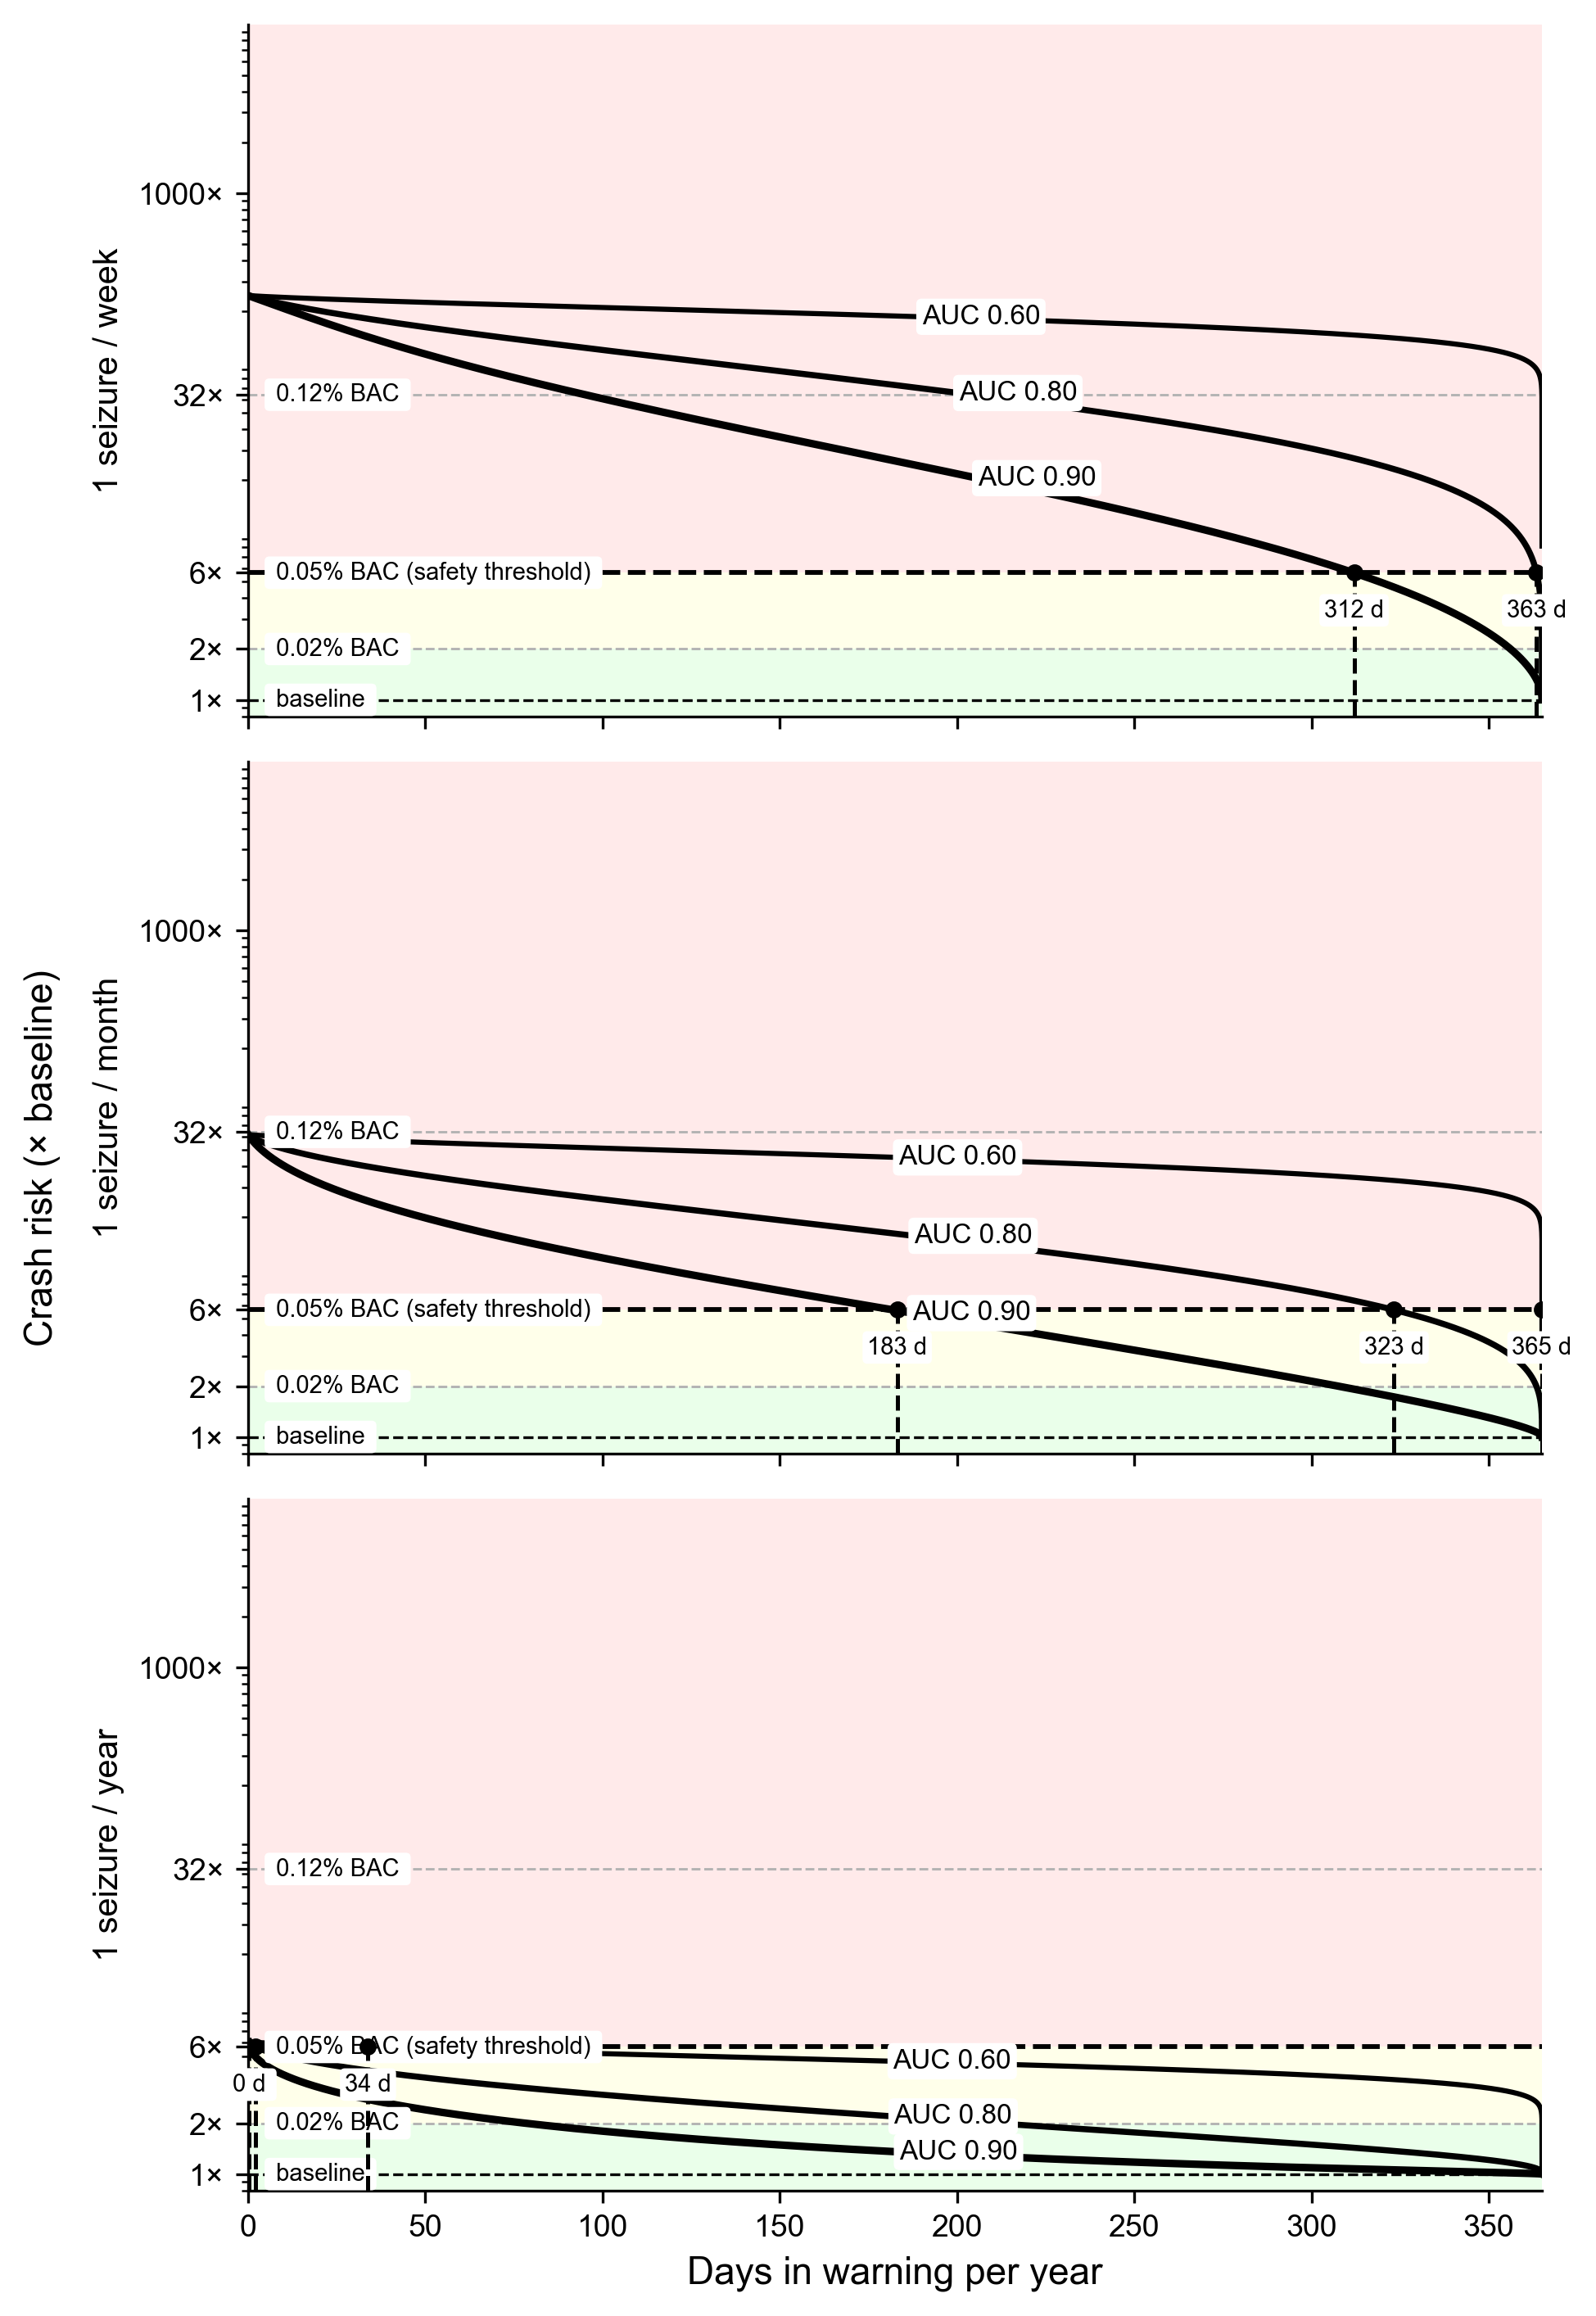
\includegraphics[width=0.85\textwidth]{Figure_S2.png}
  \caption{\textbf{Mechanism: crash risk versus days in warning.} Rows are seizure
  frequencies ($1$/week, $1$/month, $1$/year), at $1$ hr/day driving. Black curves are
  AUC $0.60$, $0.80$, $0.90$ (thicker lines indicate higher AUC). Shaded bands and
  dashed lines mark BAC-equivalent risk levels ($0.02\%$, the $0.05\%$ safety
  threshold, $0.12\%$). Black circles mark the minimum days in warning needed to reach
  the threshold.}
  \label{fig:S2}
\end{figure}

\paragraph{Key insights.}
\begin{itemize}[leftmargin=2em,itemsep=2pt]
  \item \emph{High AUC is the binding constraint.} Algorithms need AUC $\ge 0.90$ to
  provide meaningful driving days for patients with weekly or monthly seizures.
  \item \emph{Patients with rare seizures ($\le 1$/year)} are at or near unrestricted
  driving even at low AUC ($\approx 331$ days/year at AUC $0.60$), though not literally
  always-safe.
  \item \emph{Monthly seizure patients benefit greatly}: AUC $0.90$ permits
  $\approx 182$ days/year; AUC $0.95$ permits $\approx 273$.
  \item \emph{Weekly seizure patients face significant restrictions}: even AUC $0.90$
  permits only $\approx 53$ days/year; AUC $0.80$ is essentially insufficient
  ($\le 2$ days/year).
\end{itemize}

\section{Sensitivity Analyses}
\label{sec:sensitivity}

Three analyses test the robustness of the main result: to the most uncertain parameter
($q_f$, Section~\ref{sec:qf-sensitivity}), to driving duration
(Section~\ref{sec:duration}), and to ROC-curve shape (Section~\ref{sec:roc-shape}).

\subsection{Conditional Fatal-Crash Probability $q_f$}
\label{sec:qf-sensitivity}

The parameter $q_f = P(\text{fatal crash} \mid \text{seizure while driving})$ is the
model's most uncertain component; no single study directly reports it, making it an
inferred severity parameter. We examined the defensible range $q_f \in [0.005,\ 0.05]$:

\begin{itemize}[leftmargin=2em,itemsep=2pt]
\item \textbf{Lower bound ($q_f = 0.005$):} moderate crash rate ($\sim 0.30$) given a
seizure while driving $\times$ moderate case-fatality ($\sim 0.02$) --- closer to
baseline fatal-crash severity.
\item \textbf{Central ($q_f = 0.02$):} Gastaut \& Zifkin 1987 observed crash rate
($\sim 0.55$) $\times$ case-fatality of seizure-related crashes ($\sim 3$--$5\%$,
inferred from Sheth et al.\ 2004 and Drazkowski et al.\ 2003).
\item \textbf{Upper bound ($q_f = 0.05$):} counts near-misses as effective crashes
(Gastaut: $\sim 38\%$ additional near-miss rate) with upper-bound severity.
\end{itemize}

Table~\ref{tab:qf} reports driving days/year at AUC $= 0.90$, $1$\,hr/day, across the
$q_f$ range.

\begin{table}[h!]
\caption{Sensitivity of driving days/year to $q_f$ at AUC $= 0.90$, $1$\,hr/day.}
\label{tab:qf}
\centering
\begin{tabular}{lccc}
\toprule
Seizure frequency & $q_f = 0.005$ & $q_f = 0.02$ (central) & $q_f = 0.05$ \\
\midrule
$1$/week  & 154 & 53  & 20  \\
$1$/month & 314 & 182 & 99  \\
$1$/year  & 365 & 365 & 334 \\
\bottomrule
\end{tabular}
\end{table}

The amplification factor $A = q_f / (24 \lambda_f)$ ranges from $\approx 463$ (lower)
through $\approx 1852$ (central) to $\approx 4630$ (upper); the corresponding maximum
tolerable $P(\text{seizure} \mid \text{forecast safe})$ for $\mathrm{RR} \le T = 5.66$
ranges from $\approx 1.0\%$ down to $\approx 0.10\%$.

\begin{figure}[h!]
  \centering
  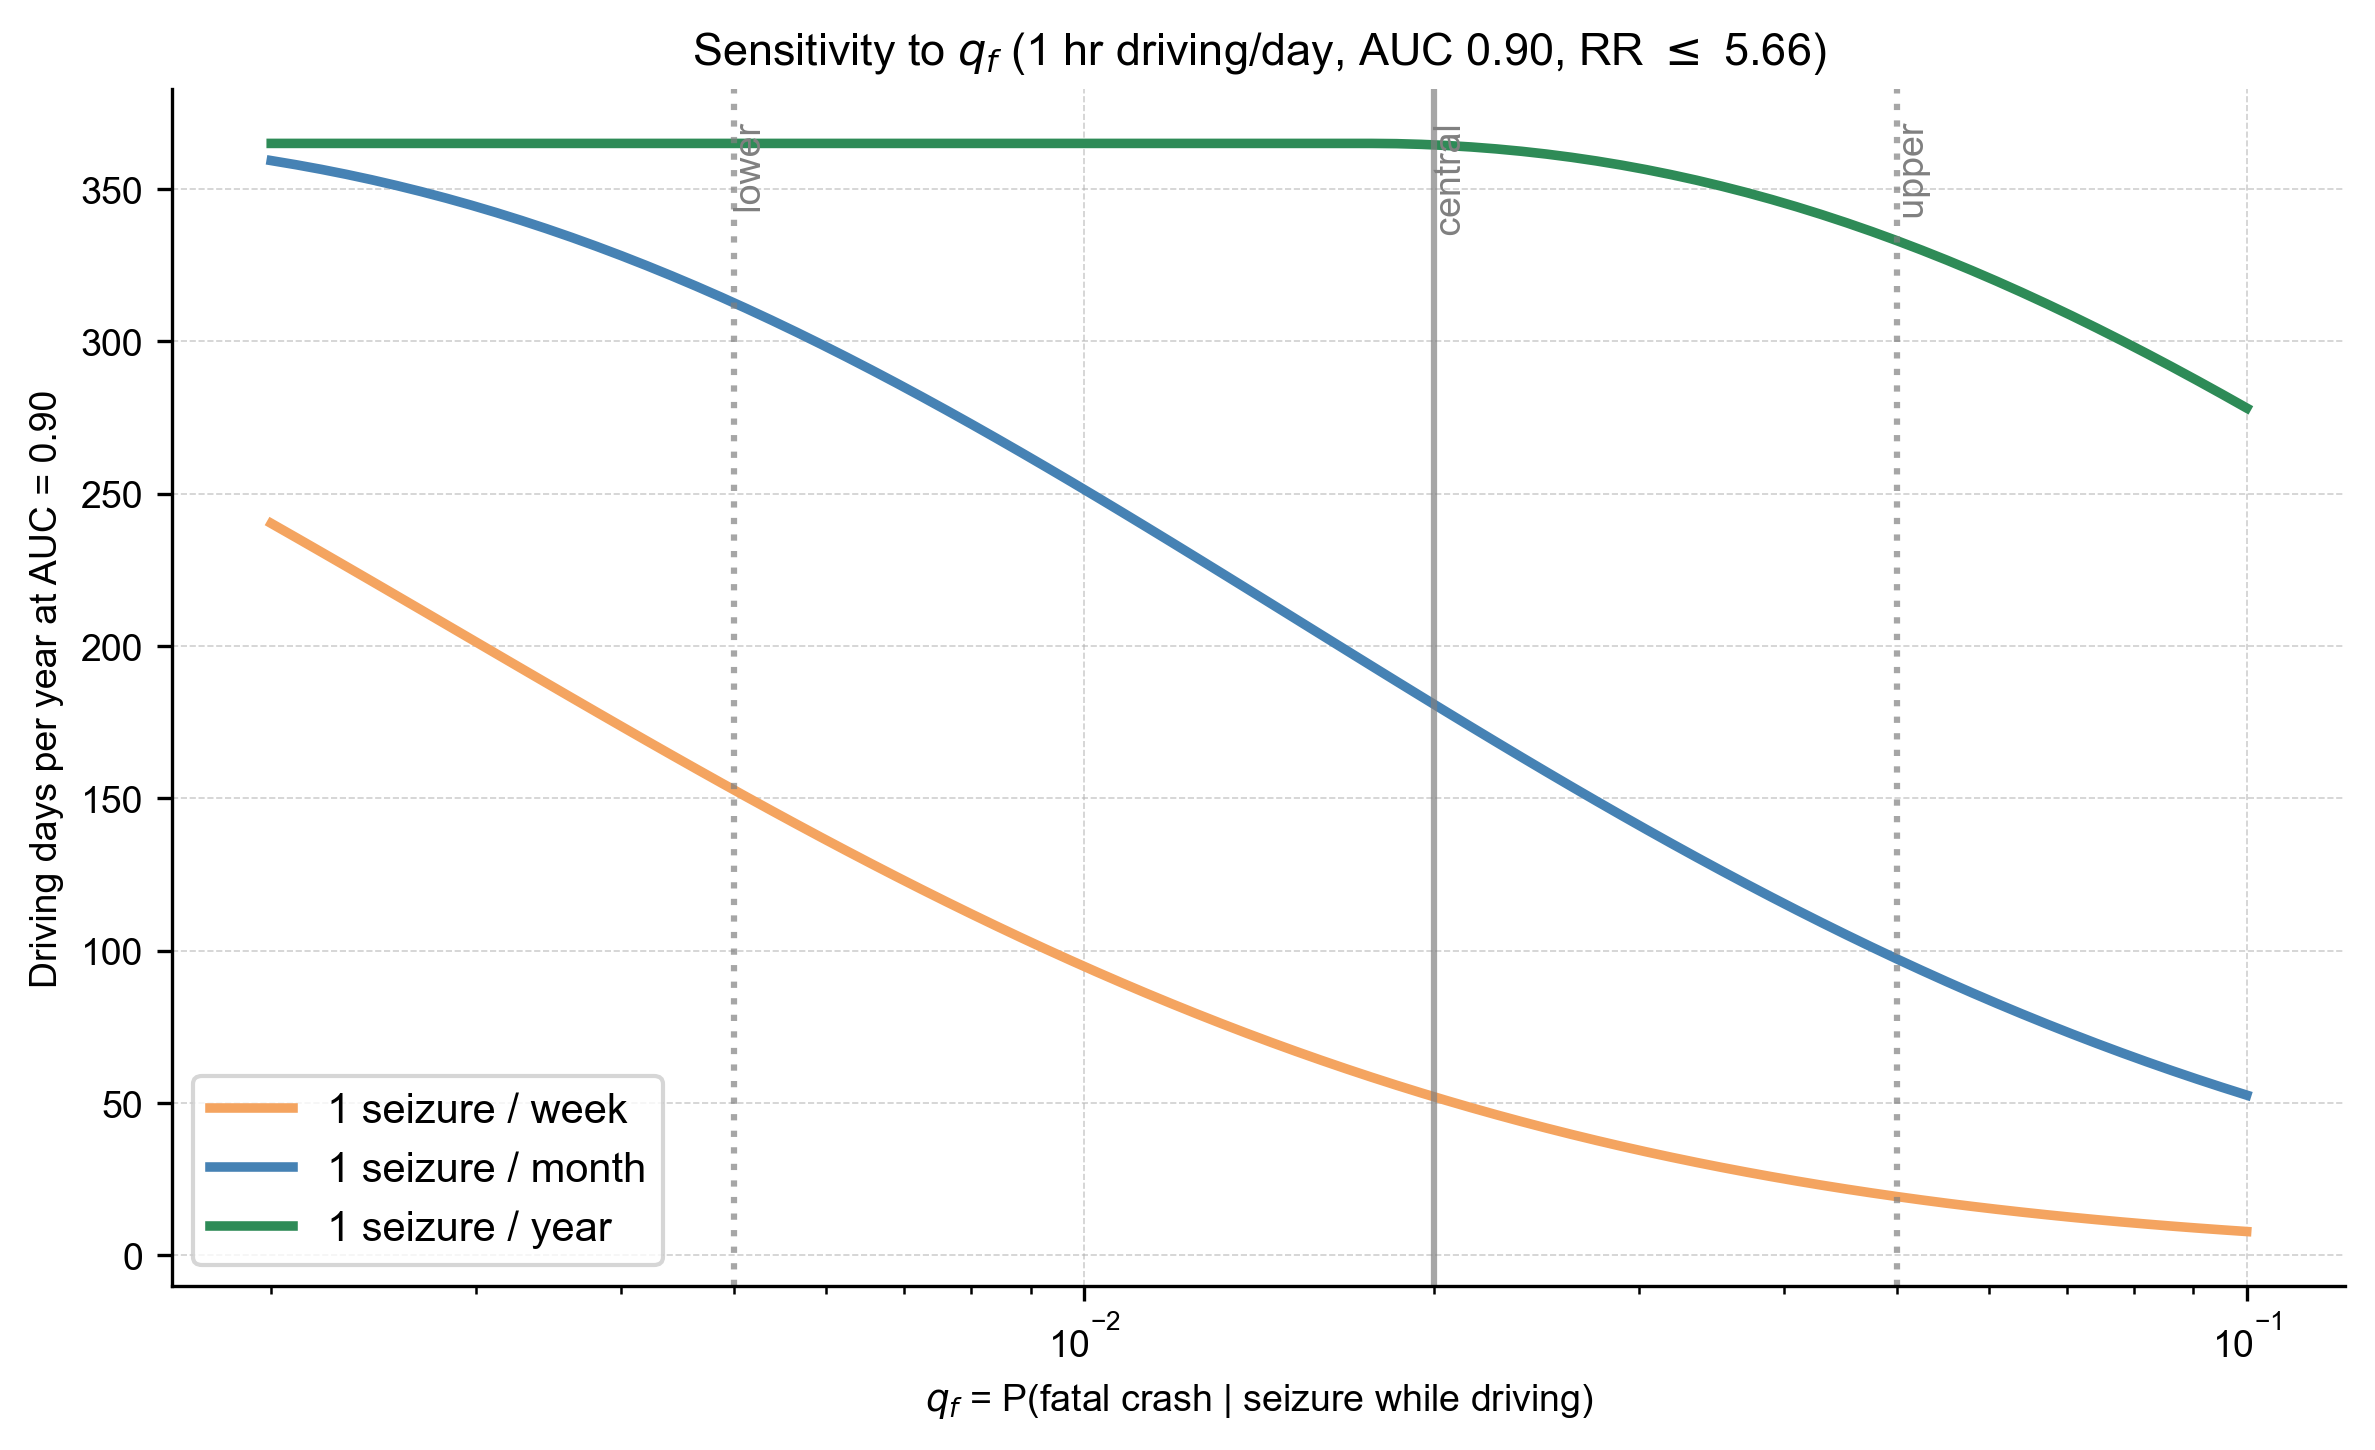
\includegraphics[width=0.85\textwidth]{Figure_S3.png}
  \caption{\textbf{Sensitivity of driving days to $q_f$.} Driving days per year at
  AUC $= 0.90$ and $1$\,hr/day, as a function of $q_f$. Vertical guides mark the
  lower bound ($0.005$), the central estimate ($0.02$), and the upper bound ($0.05$).}
  \label{fig:S3}
\end{figure}

\paragraph{Interpretation.}
Across the full range, the qualitative finding holds: weekly-seizure patients cannot
achieve unrestricted driving even at AUC $0.90$, and yearly-seizure patients remain
at or near unrestricted driving. The quantitative allowance for monthly seizures spans
roughly a factor of three. Until empirical data better anchor the parameter,
stakeholders may prefer the conservative-end $q_f = 0.05$.

\subsection{Driving Duration (Exposure Invariance)}
\label{sec:duration}

Section~\ref{sec:crash-risk} shows analytically that relative risk is approximately
invariant to driving duration $D$, because both seizure-related and baseline fatal
risks scale with exposure (Equation~\ref{eq:rr-approx}). This invariance also holds
numerically: driving-day allowances coincide to integer rounding across the examined
durations (Table~\ref{tab:duration}).

\begin{table}[h!]
\caption{Driving days/year coincide across exposure levels under the relative-risk
benchmark.}
\label{tab:duration}
\centering
\begin{tabular}{llccc}
\toprule
Seizure frequency & AUC & $30$ min/day & $1$ hr/day & $2$ hr/day \\
\midrule
$1$/week  & $0.90$ & 53  & 53  & 53  \\
$1$/month & $0.90$ & 182 & 182 & 182 \\
$1$/year  & $0.80$ & 363 & 363 & 363 \\
\bottomrule
\end{tabular}
\end{table}

Absolute fatal-crash risk does still scale with driving duration; an alternative
\emph{absolute}-risk benchmark would depend directly on exposure. Under the
relative-risk benchmark used here, driving duration is not a material determinant of
the allowable driving days.

\subsection{ROC Curve Shape}
\label{sec:roc-shape}

The equal-variance binormal assumption implies a specific sensitivity--specificity
relationship. Real ROC curves can deviate from this relationship due to unequal
variances (S-shaped), mixture distributions (hooked; some seizures easier to predict
than others), or finite-sample effects. We test three score-generating models, all
calibrated to $\mathrm{AUC} \approx 0.90$.

\paragraph{Equal-variance binormal} (baseline): negatives follow $N(0,1)$ and positives
follow $N(m,1)$, with $m = \sqrt{2}\,\Phi^{-1}(0.90) \approx 1.81$.
Equations~(\ref{eq:sensitivity})--(\ref{eq:fpr}) give sensitivity and FPR.

\paragraph{Unequal-variance binormal} (S-shaped): negatives $N(0,1)$, positives
$N(\mu_1, \sigma_1)$ with $\mu_1 = 2.4$, $\sigma_1 = 1.4$. For threshold $t$,
\begin{equation}
\mathrm{Sensitivity} \;=\; 1 - \Phi\!\left(\frac{t - \mu_1}{\sigma_1}\right),
\qquad
\mathrm{FPR} \;=\; 1 - \Phi(t).
\label{eq:unequal-var}
\end{equation}
On forecast-safe days, the posterior substitutes
$\Phi\!\left((t - \mu_1)/\sigma_1\right)$ for $\Phi(t - m)$ in
Equation~\ref{eq:posterior}.

\paragraph{Mixture model} (hooked): negatives $N(0, 1)$, positives
$w\,N(\mu_{\text{easy}}, 1) + (1 - w)\,N(\mu_{\text{hard}}, 1)$, with $w = 0.7$,
$\mu_{\text{easy}} = 2.5$, $\mu_{\text{hard}} = 0.8$. From this mixture,
\begin{equation}
\mathrm{Sensitivity}
\;=\; w\,[1 - \Phi(t - \mu_{\text{easy}})] \;+\; (1 - w)\,[1 - \Phi(t - \mu_{\text{hard}})],
\label{eq:mixture-sens}
\end{equation}
\begin{equation}
P(S < t \mid \text{seizure})
\;=\; w\,\Phi(t - \mu_{\text{easy}}) \;+\; (1 - w)\,\Phi(t - \mu_{\text{hard}}).
\label{eq:mixture-belowt}
\end{equation}

\begin{figure}[h!]
  \centering
  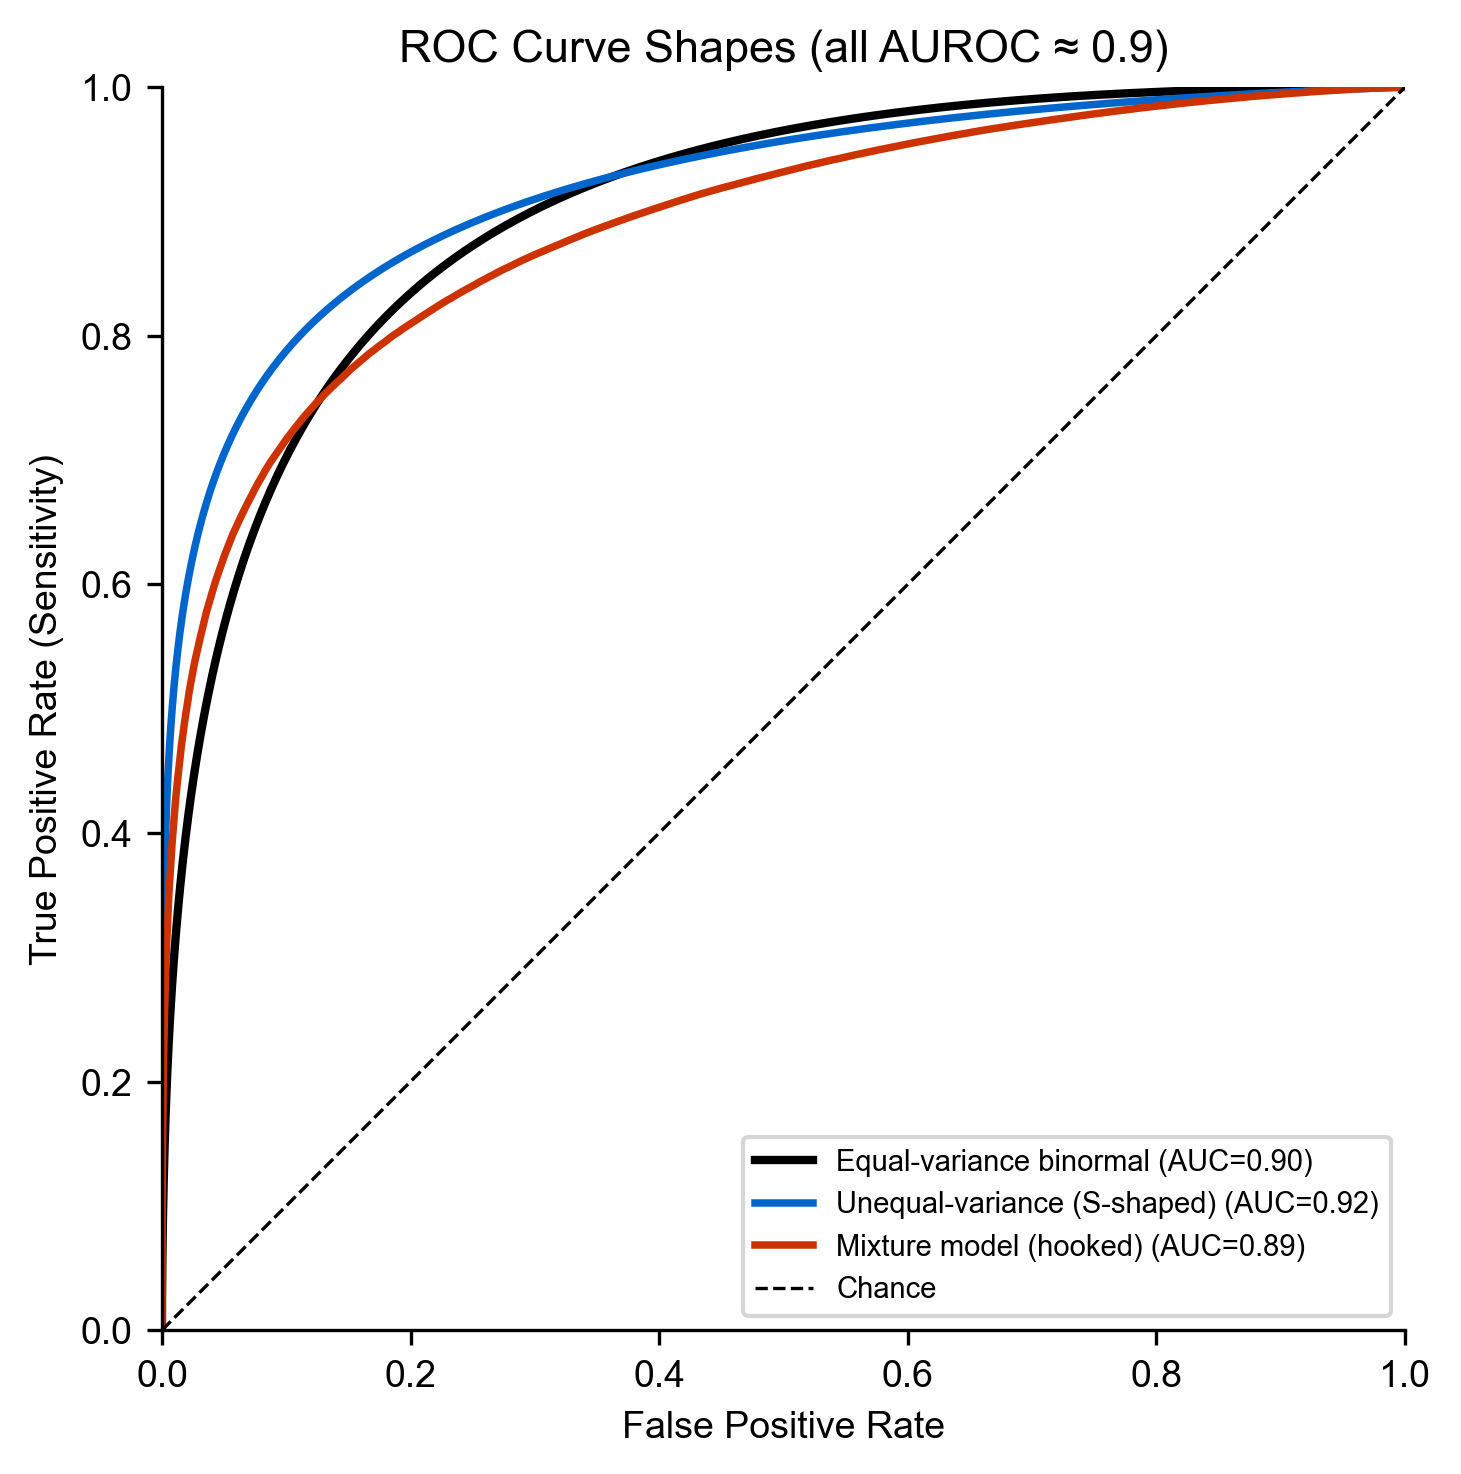
\includegraphics[width=0.55\textwidth]{Figure_S4.png}
  \caption{\textbf{Three ROC curve shapes}, all at $\mathrm{AUC} \approx 0.90$.
  Equal-variance binormal (black, central), unequal-variance/S-shaped (blue, top-left),
  and hooked mixture model (red).}
  \label{fig:S4}
\end{figure}

Table~\ref{tab:roc-shape} reports driving days at $\mathrm{AUC} \approx 0.90$ and
$1$\,hr/day for each ROC shape; Figure~\ref{fig:S5} shows the corresponding
crash-risk-versus-warning-days curves across shapes and seizure frequencies.

\begin{table}[h!]
\caption{Driving days/year at $\mathrm{AUC} \approx 0.90$, $1$\,hr/day, by ROC shape.}
\label{tab:roc-shape}
\centering
\begin{tabular}{lccc}
\toprule
Seizure frequency & Equal-variance binormal & S-shaped (unequal var.) & Hooked (mixture) \\
\midrule
$1$/week  & 53  & Cannot reach safety & 1   \\
$1$/month & 182 & 145                 & 66  \\
$1$/year  & 365 & 365                 & 365 \\
\bottomrule
\end{tabular}
\end{table}

\begin{figure}[h!]
  \centering
  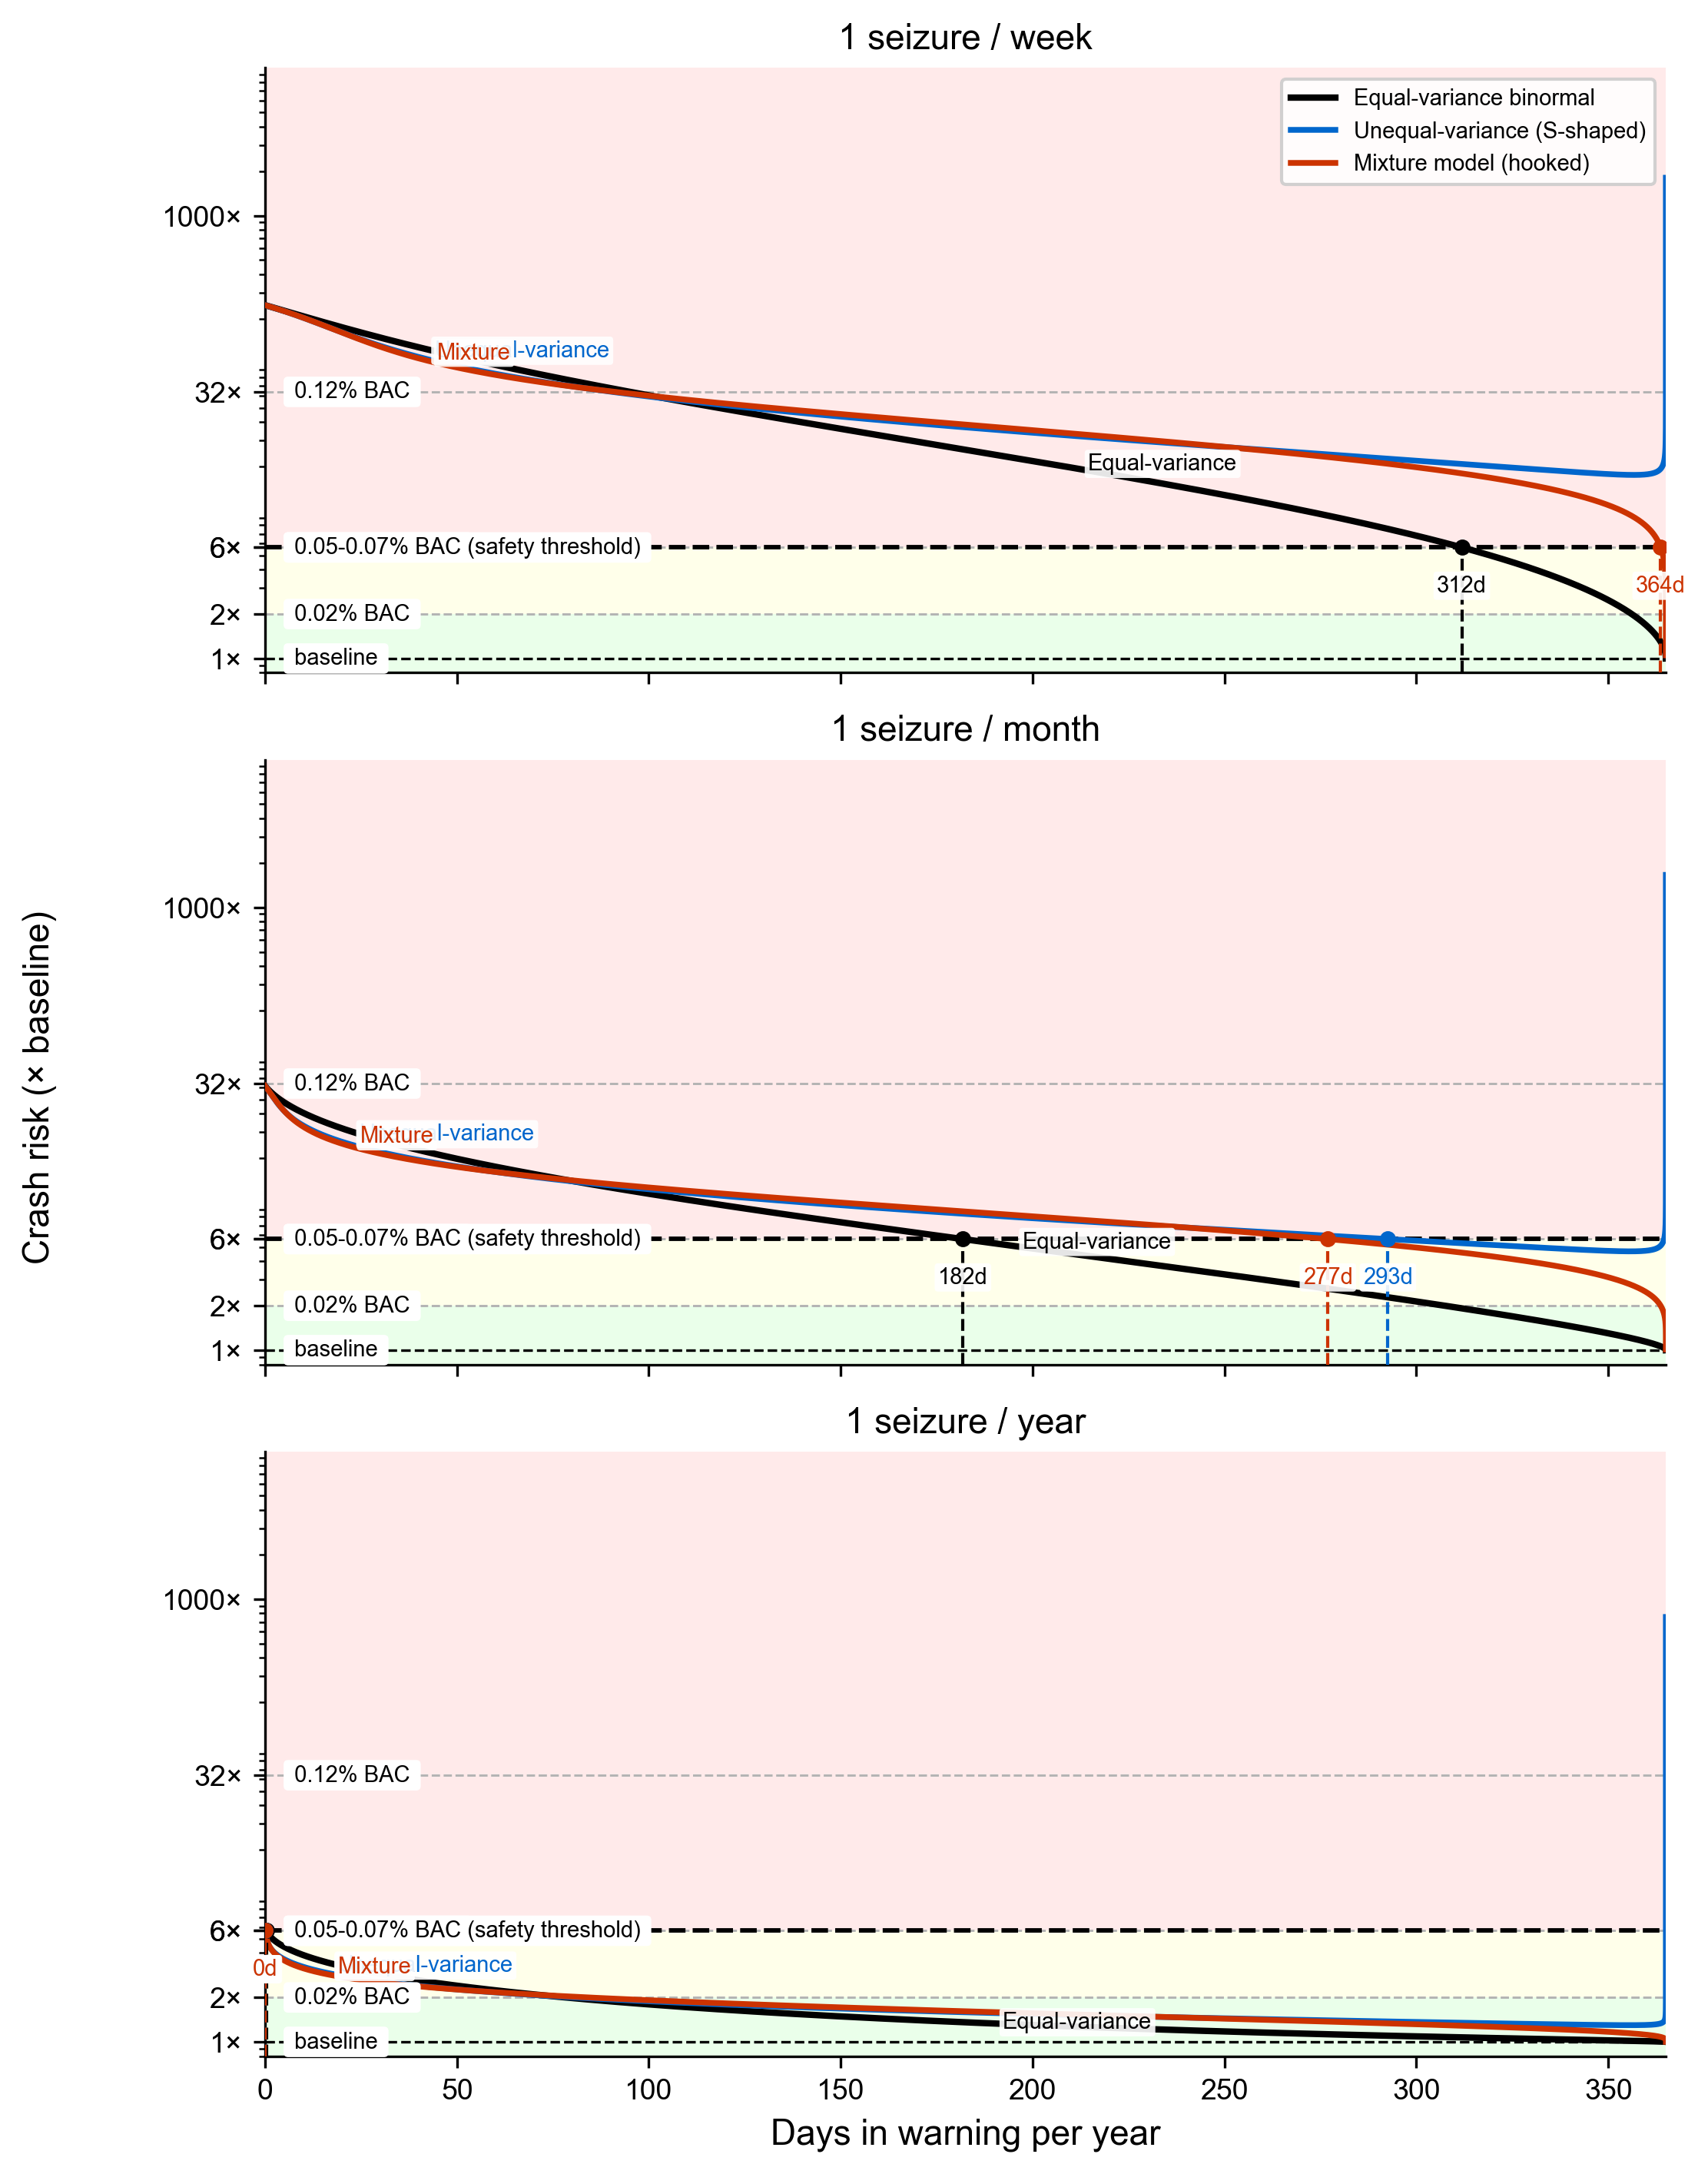
\includegraphics[width=0.7\textwidth]{Figure_S5.png}
  \caption{\textbf{Crash risk versus days in warning for three ROC shapes}, by seizure
  frequency, at $1$\,hr/day and $\mathrm{AUC} \approx 0.90$. Equal-variance binormal
  (black), S-shaped (blue), and hooked mixture (red). Black dashed line: safety
  threshold.}
  \label{fig:S5}
\end{figure}

\paragraph{Findings.}
\begin{itemize}[leftmargin=2em,itemsep=2pt]
  \item \emph{At high seizure frequencies, ROC shape matters.} Equal-variance binormal
  is the most optimistic shape; the S-shaped form fails to reach the threshold at all
  for weekly seizures, and the hooked mixture model permits only $1$ day. For monthly
  seizures, the spread is $182\to 145\to 66$ days/year.
  \item \emph{At low seizure frequency (yearly), shape is irrelevant} --- all three ROC
  families permit essentially full-year driving because the prior seizure probability
  is already very low.
  \item \emph{Net.} AUC remains the primary determinant, but ROC geometry is a
  meaningful secondary factor. Because equal-variance binormal is the most optimistic
  of the three, real-world (S-shaped or hooked) ROCs at the same AUC will generally
  permit \emph{fewer} driving days than the main result suggests --- so reporting AUC
  alone may overstate clinical utility for patients with frequent seizures. The
  qualitative conclusion (high AUC is necessary, and even AUC $0.90$ is borderline for
  weekly seizures) is robust to shape.
\end{itemize}

\section{Assumptions, Limitations, and Recommendations}
\label{sec:assumptions}

\paragraph{Why the binormal model is a reasonable base case.}
It is a standard approximation in diagnostic testing and signal-detection theory, is
mathematically tractable (closed-form, reproducible), and for a given AUC tends to
offer near-best-case sensitivity-specificity trade-offs --- giving the forecasting
algorithm the benefit of the doubt. The paper's question is ``what level of performance
(AUC) is needed for safe driving decisions?'', not ``how does one specific empirical
ROC curve perform?''. Section~\ref{sec:roc-shape} quantifies the effect of departures
from this assumption.

\paragraph{Driving-exposure assumptions.}
\begin{enumerate}[leftmargin=2em,itemsep=2pt]
  \item \textbf{Seizure timing is uniformly distributed} over the $24$-hour day. Many
  patients have circadian patterns (nocturnal epilepsy, morning clustering); the model
  is conservative for seizures concentrated outside driving hours and optimistic for
  daytime clustering.
  \item \textbf{Driving duration is constant across days.} Real driving varies; the
  $30$ min/day--$2$ hr/day range brackets typical commuter and heavy-driver patterns
  (and, per Section~\ref{sec:duration}, barely affects the relative-risk result).
  \item \textbf{$q_f = 0.02$ is an inferred severity parameter} (range $0.005$--$0.05$),
  decomposing as $P(\text{crash} \mid \text{seizure while driving}) \approx 0.55$
  (Gastaut \& Zifkin 1987) $\times$ case-fatality $\approx 3$--$5\%$ (inferred from
  Sheth et al.\ 2004 and Drazkowski et al.\ 2003). It depends on seizure type, aura,
  road conditions, and vehicle safety features; Section~\ref{sec:qf-sensitivity}
  reports the sensitivity analysis.
\end{enumerate}

\paragraph{Recommendations for algorithm developers.}
\begin{enumerate}[leftmargin=2em,itemsep=2pt]
  \item Aim for AUC $\ge 0.90$ as a minimum for driving applications.
  \item Characterise your empirical ROC shape --- an S-shaped or hooked curve at the
  same AUC permits fewer driving days and shifts optimal operating points.
  \item For patients with frequent seizures, even AUC $= 0.90$ may be insufficient for
  practical driving policies.
  \item For patients with rare seizures, forecasting may be unnecessary for safety;
  focus on other quality-of-life benefits.
  \item Consider patient-specific seizure frequency and driving patterns when
  counselling about risk.
\end{enumerate}

\section{Reproducibility}
\label{sec:reproducibility}

All calculations use closed-form expressions implemented with NumPy, SciPy
(\texttt{scipy.stats.norm} for the Gaussian CDF/inverse CDF), and Matplotlib.

\begin{verbatim}
pip install numpy matplotlib scipy
jupyter notebook crashes_vs_TiW.ipynb        # interactive
# or run all cells programmatically:
jupyter nbconvert --to notebook --execute crashes_vs_TiW.ipynb
\end{verbatim}

\begin{table}[h!]
\caption{Notebook cell layout and outputs.}
\label{tab:cells}
\centering
\begin{tabular}{cl}
\toprule
Cell & Produces \\
\midrule
0 & Figure S2 --- crash risk vs.\ days in warning ($3$ frequencies, $1$ hr/day) \\
1 & Figure 1 --- driving days vs.\ AUC (main result) \\
2 & Figure S1 --- binormal model schematic \\
3 & Figures S4 \& S5 --- ROC shape geometries and sensitivity \\
4--5 & Extended AUC table (tab-delimited, all frequencies/durations) \\
6 & Figure S3 --- $q_f$ sensitivity \\
\bottomrule
\end{tabular}
\end{table}

Figure files are produced as PDF and PNG: \texttt{Figure\_1}, \texttt{Figure\_S1}--\texttt{Figure\_S5}.

\end{document}
